\section{First Model and Architecture} \label{sec: first model and architecture MR}
The predefined structures, as they were mentioned in \secreff{subsec: first model and architecture}, form the base of these model types \ie a rule set was given which is equivalent to a graphical model, where the rules describe the edges. The training data was composed by randomly choosing one of the five rules and the input as well as the output word. The Neural Network was quite shallow because it contained only one hidden layer.
By using eight words from each class, the rules are easily learned (\figref{\ref{fig: first model tpm and mds}}).
\begin{figure}
	\centering
		\subcaptionbox{Learned Successor Representation of a tailored \cognitiveroom{} with apparent future states.}{
			\includegraphics[height=\twocolpicheight]{chapter4/chapter4.1/first_models/4Rules/plots/First Model + More Rules_100E_100BS_1L_1C/Transition_Probability_Matrix;_t=1,_DF=0.5.png}
		}
		\hfill
		\subcaptionbox{\gls{mds} plot of the \gls{sr} in (a) showing decent clusters.}{
			\includegraphics[height=\twocolpicheight]{chapter4/chapter4.1/first_models/4Rules/plots/First Model + More Rules_100E_100BS_1L_1C/MDS_of_Transition_Probability_Matrix;_t=1,_DF=0.5.png}
		}
	\caption{Clearly visible are the successor positions of the states \eg \texttt{Adjective → Noun}. \texttt{Nouns} are smeary because the rule set in \secreff{enum: rule set} doesn't provide one starting with \texttt{Noun}, so the Neural Network has to guess in less definite scenarios. Although there is a prediction made for each single word \ie state in the \cognitiveroom{}, only word classes are displayed to avoid clutter (Pers. Pr. = \texttt{Personal Pronoun}, Pos. Pr. = \texttt{Possessive Pronoun}).}
	\label{fig: first model tpm and mds}
\end{figure}
Since the rows encode the states, it is expected in the terms of the successor representation that the next position shows a high activation. Checking this behavior is simple because the environment (\secreff{subsec: first model and architecture}) is clearly defined. The \texttt{Noun} part of \figref{\ref{fig: first model tpm and mds}} is smeary because there is no rule for a consecutive state (in graph theory it corresponds to a sink). The undefined behavior is also revealed in the \gls{mds} illustration, where all nouns are distributed between the other word classes. By calculating the \gls{sr} for additional time steps, the result incorporates all following rules or states (\figref{\ref{fig: first model sr t=3, df=0.5}}). These matrices are interesting for analyzing the value function $ V $ (\equref{\eqref{eq: v with sr-matrix}}), which is beyond the scope of this work.
\begin{figure}
	\centering
		\subcaptionbox{Calculated \gls{sr} of a tailored \cognitiveroom{} for $ t = 2 $ and $ \gamma = 0.5 $ using the matrix of \figref{\ref{fig: first model tpm and mds}}.}{
			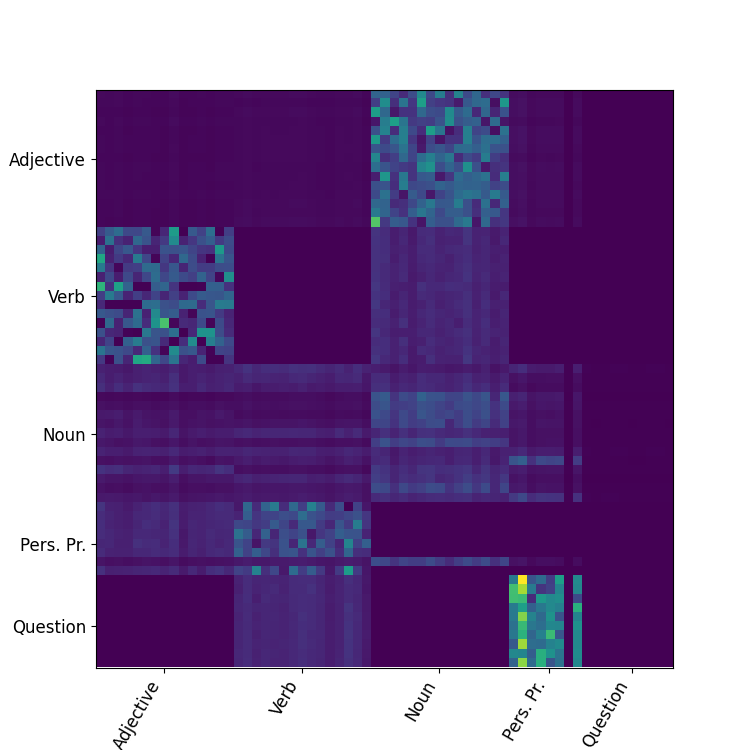
\includegraphics[height=\twocolpicheight]{chapter4/chapter4.1/first_models/4Rules/plots/First Model + More Rules_100E_100BS_1L_1C/SR,_t=2,_DF=0.5.png}
		}
		\hfill
		\subcaptionbox{\gls{mds} plot of the \gls{sr} in (a) with properly grouped word classes}{
			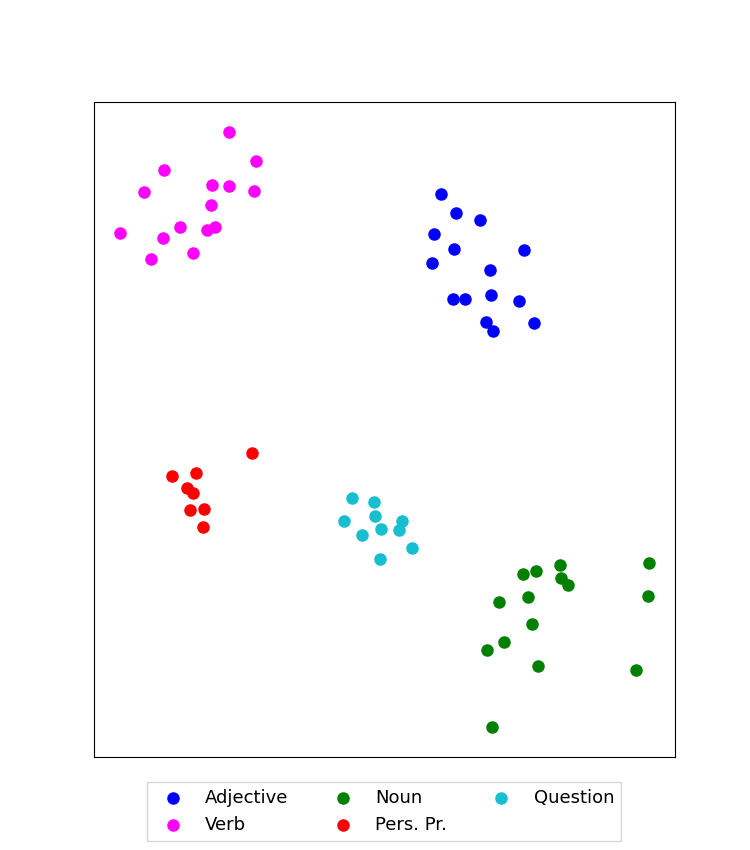
\includegraphics[height=\twocolpicheight]{chapter4/chapter4.1/first_models/4Rules/plots/First Model + More Rules_100E_100BS_1L_1C/MDS_of_SR,_t=2,_DF=0.5.png}
		}
	\caption{Calculating the Successor Representation for a higher time step \ie $ t=2 $, already demonstrates the properties of the construction. For all states (visual aggregated into the word class), it is possible to derive successor states \eg the two step rule \texttt{Question → Pers. Pr. → Verb}.}
	\label{fig: first model sr t=3, df=0.5}
\end{figure}
%The \gls{sr} doesn't serve the purpose of predicting future states because then the plot in \figref{} would be misleading. In this case it suggests staying in the \texttt{Pronoun} state after $ t = 3 $ which is impossible because pausing \eg \texttt{Pronoun → Pronoun} is no valid rule. And also reentering the state after leaving it is no option since \texttt{Question} is the single possibility for transiting \texttt{Pronoun} but \texttt{Question} has no predecessor. The \gls{sr} has to be read in terms of the value function $ V $ in \eqref{eq: v with sr-matrix}.

\bigskip
% \TODOL{Aufzählung im Moment aufgeteilt, muss nicht sein. Evtl. doch wieder in den Fließtext.}
The principle also works out when using more rules and a larger data set. The enhancement is done by introducing four new rules
\begin{itemize}
	\item \texttt{Question word → Verb}
	\item \texttt{Noun → Personal Pronoun}
	\item \texttt{Adverb → Possessive Pronoun}
	\item \texttt{Personal Pronoun → Adverb},
\end{itemize}
more words for the already existing categories and two new word classes (\texttt{Adverb} and \texttt{Possessive Pronoun}). The result in \figref{\ref{fig: more rules and word tpm and mds}} is in clarity similar to \figref{\ref{fig: first model tpm and mds}} but without having an obvious blurry row, even though the word class \texttt{Possessive Pronoun} is without successor as \texttt{Noun} in the trial before. Nevertheless, some similarities to \texttt{Question word} were detected. The only characteristic they seem to share is having exactly one edge. Also, clusters are in the \gls{mds} apparent, indicating learning worked. Although artificial, conceptually they serve as a standard to reach for the upcoming configurations.
\begin{figure}
	\centering
		\subcaptionbox{\gls{sr} of a more advanced model.}{
			\includegraphics[height=0.375\textheight]{chapter4/chapter4.1/first_models/8Rules/plots/First Model + More Rules_100E_100BS_1L_1C/Transition_Probability_Matrix;_t=1,_DF=0.5.png}
		}
		\hfill
		\subcaptionbox{\gls{mds} plot of (a).}{
			\includegraphics[height=0.375\textheight]{chapter4/chapter4.1/first_models/8Rules/plots/First Model + More Rules_100E_100BS_1L_1C/MDS_of_Transition_Probability_Matrix;_t=1,_DF=0.5.png}
		}
	\caption{The illustrated plots stem from a model using additional rules backed by more word classes and a larger database to retrieve the training data. The outcomes are similar to \figref{\ref{fig: first model tpm and mds}}. The upcoming states are obvious. The model can handle ambiguous successors \eg \texttt{Personal Pronoun → Verb} and \texttt{Personal Pronoun → Adverb} are deployed rules.}
%		Learned Successor Representation (left) and corresponding \gls{mds} plot (right) of a more advanced model consisting of eight rules backed by a larger variety of words used for training.}
	\label{fig: more rules and word tpm and mds}
\end{figure}
